
\section{Discussion and Research Gap}

% Chapter 4
% ======================================================================================================
% NOTES, TODOS
% limitation 
% Observation -> blockchain for data integrity and sharing Machine learning for intrusion detection cloud -> deploying dt in cloud 
% Privacy preserving 
% DT is a simulation platform 
% ======================================================================================================

In this literature review part of the project, we conducted a systematic way of reviewing the literature on the use of Digital Twin technology in Industry 4.0 domain to enhance security requirements. The study was carried out using the three-phase approach of conducting a systematic literature review that includes designing a review protocol, conducting a review, and analysis. The aim was to investigate how Digital Twin is used to enhance security Industry 4.0. Besides, we explore the literature on what security scheme or mechanism is used to protect the integrity and confidentiality of data flow between (I)IoT devices and Digital Twin.


A total of 727 articles were identified from online digital databases, such as ScienceDirect, SpringerLink, Scopus, IEEExplore, ACM, and Web of Science. After applying inclusion and exclusion criteria and removing duplicates, we left with 67 research papers in which we perform analysis to answer our research questions.

Research studies on the use of Digital Twin as a security solution were started published in 2018. Since then it has been observed that the adoption of Digital Twin technology is growing rapidly in various Industry 4.0 sectors leading to a significant surge in research articles over the past 6 years particularly in years 2021 and 2022. 

The contributions of the research vary from theoretical concepts to Digital Twin-based security platforms. Though the majority of the studies focus on providing a framework with theoretical concepts.

In the following section we discuss, first the past, present and future status of Digital Twin. Then, we briefly look into how Digital Twin is used as a security tool. Finally, we reflect on security mechanisms discussed in the literature for protecting data flow between Digital Twin and (I)IoT.

\subsection{Observation and Findings}
As a result of a thorough review of the literature on the use of DT technology for securing (I)IoT applications and securing digital communication between DT and IoT devices, few findings have been identified.


\subsubsection*{Past, Present, and Future of Digital Twin}
In its early days, the Digital Twin concept was used primarily as a model in the manufacturing industry. However, with the advent of enabling technologies such as (I)IoT, AI, and cloud computing, it has evolved into an integrated platform capable of providing a range of services beyond just modelling. Today, it is used in various industries to enhance the security of complex environments in addition to improving productivity and efficiency. Looking ahead, digital twins are expected to incorporate even more technologies and integrate more deeply with humans through research on Human-Computer Interaction technology. 

\begin{figure}[H]
    \centering
    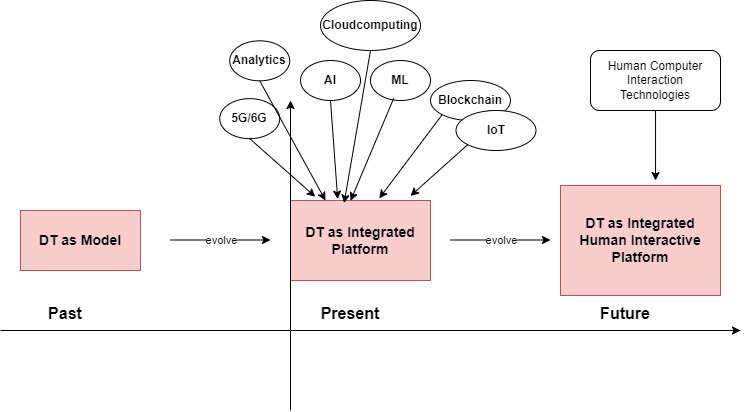
\includegraphics[width=\textwidth]{images/rt/dt-evolution.drawio.png}
    \caption{Evolution of Digital Twin Over Time}
    \label{fig:dt-evol}
\end{figure}


% \textbf{\textit{DT as integrated platform}}:
From the review, we identified Digital Twin as an integrated platform of a virtual model and enabling technologies to process collected data from the operating environment through (I)IoT sensors in order to gain insight for monitoring, optimization, and security purposes. 

One crucial aspect emphasized by authors for proper functioning Digital Twin deployment is the necessity for real-time and uncorrupted data. Our proposed solution, based on a lightweight and authenticated encryption algorithm, ensures that this requirement is met. The data communicated between Digital Twin and resource-constrained (I)IoT device is secured its integrity (with authentication) and confidentiality (with encryption). 



\subsubsection*{Digital Twin as security tools}
Digital Twin is being developed to be used for various purposes, including security. Our review indicates it is mostly used as a simulation platform for conducting testing and training. Next to using DT as a simulation, a number of solutions are proposed to detect anomalies \cite{chukkapalliCyberPhysicalSystemSecurity2021} and intrusions in cyber-physical systems(CPS) and industrial control systems (ICS) \cite{vargheseDigitalTwinbasedIntrusion2022, akbarianIntrusionDetectionDigital2020}. In this regard, the potential threats are DDoS, botnet activities, network breaches, and anomaly processes.   


The majority of papers discuss setting up a digital twin in a standalone environment to enhance the security of a targeted industry \cite{almeaibedDigitalTwinAnalysis2021, veledarDigitalTwinsDependability2019, chukkapalliCyberPhysicalSystemSecurity2021, adrienbacueDigitalTwinsEnhanced2022}. However, we have found a few papers that present the idea of sharing cyber threat intelligence(CTI) \cite{dietzHarnessingDigitalTwin2022, almeaibedDigitalTwinAnalysis2021} data generated using Digital Twin across industries to collectively improve security. This is a unique approach to using digital twin technology that could have a significant impact on tackling big security problems, such as ransomware through sharable CTI. However, for this to be effective, we argue that the data-sharing process must be in real-time with privacy in mind. 


In terms of enabling technology, machine learning and data analytics are the core technology used to power up Digital Twin to function as a security-enhancing tool. In other words, detection and protection security services are realized mainly using machine learning and data analytics that operate on large data collected through sensors. 


\subsection{Research Gap}
\label{sec:gap}
% \item\textbf{\textit{Lack of discussion on Lightweight encryption}}: 

In our review of selected papers, it became evident that most of the papers place little emphasis on ensuring the authenticity and integrity of the sensor data that is fed into the Digital Twin. Even though a handful of papers discuss securing the data transmission channel, their recommendations rely on traditional encryption and authentication mechanisms such as AES, SHA-256 and RSA. 

This is concerning because in most use cases data generating sensors are power constraints where it is not feasible to deploy traditional encryption algorithms to secure them. Hence, it is important to focus on lightweight algorithms to protect data confidentiality, integrity and authenticity of data used in Digital Twin-based solutions.



\subsection{Future Directions}

The application Digital Twin for security is in Industry 4.0 at its early stage. While researchers have made significant contributions to its development, there are still gaps that require exploration and improvement. In this section, we identify and discuss three potential areas of research.

\textbf{\textit{Efficient lightweight encryption algorithms}}: As the development of Digital Twin technology progresses, it is expected that it will become accurate in replicating physical objects and processes. To achieve this level of accuracy, a large number of tiny, resource-constrained IoT sensors will need to be deployed on a massive scale to measure every aspect of the physical status being replicated. This presents future research directions for designing and implementing efficient encryption algorithms that can be deployed on resource-constrained devices.


% \textbf{\textit{Machine learning}}: Artificial intelligence(AI) is expected to play a crucial role in the future development of DT technology. Specifically, there are two potential areas where AI can be utilised: to perform analytics on collected data and to create AI-enabled simulations. Hence, future research could explore how machine learning technology is used in conjunction with DT models. This could involve conducting a systematic literature review to better understand how machine learning has been integrated within DT technology in previous research studies.

\textbf{\textit{Remote access control for DT}}: One area of research that we have identified as a gap in the literature is the secure remote access control to the virtual counterpart of an ICS component for vendors to perform troubleshooting and testing. In the traditional real-world industry setup, vendors of ICS components have remote access control to the physical object of the industry for various reasons. However, it is not clear how this is going to be handled on the DT yet. One potential direction for research is to explore and investigate how secure remote access can be achieved to one or more components of the DT.

% \textbf{\textit{DT based ransomware detection}}
\textbf{\textit{Human computer interaction}}: Finally, future research could explore the human-computer interaction (HCI) aspect of DT technology. This could involve examining how users interact with DT models and exploring new and innovative ways to improve the user experience. By improving the HCI aspect of DT technology, it may be possible to enhance the accuracy and reliability of the models by ensuring that human error is minimized.

\subsection{Limitations Of The Study}
% The concept of DT definition are not complete  
% Most study are focused on farmework 
% 
This study has two main categories of limitations: those related to collecting searching papers and those related to reviewing them.

\textbf{\textit{Limitation related searching}}: Regarding the limitations related to collecting papers, the first issue is with the methodology used to select papers. Only papers with the exact phrase "[Dd]igital [Tt]win[s]?" in their title were collected for review. While the authors argue that research focused on digital twins will likely use this term in the title, this is not always the case. However, this approach also had the benefit of limiting the number of papers reviewed to those specifically discussing digital twins in security, which could otherwise have been a much larger pool. 

% Another limitation within this category is related to the three-stage searching mechanism employed to query papers from online archives. In one of the databases, we were unable to use the methodology directly as it lacked dedicated fields for searching the "abstract" sections of papers, unlike in the other libraries. However, we attempted to retrieve all papers with "digital twin*" in their title and at least one of the terms "security," "industry," or "IoT" and manually screened them to filter out the relevant ones.

\textbf{\textit{Limitation related to reviewing}}: The limitations associated with the process of reviewing papers are described as follows. First, the majority of papers fail to provide a complete and comprehensive definition of Digital Twin. Specifically, while the "state" component -- encompassing both the virtual and physical states -- is often explicitly described, the intended purpose and interconnectivity between these states are not consistently included in the definition.

Another limitation within this category relates to the misunderstanding of Digital Twin with simulation software. Few papers, particularly within the healthcare sector, propose solutions utilizing simulation software under the consideration of Digital Twin. This can lead to confusion and potentially incorrect conclusions regarding the potential benefits and drawbacks of Digital Twin technology.

 Lastly, it has been observed that there is inconsistency in the usage of the terms Framework, Methodology, and Architecture, which are often used interchangeably without a clear understanding of their definitions and distinctions. The authors argue that this could be due to a lack of consensus on how these terms should be used to categorize the contributions of authors. This inconsistency is particularly evident in cases where different terms are used to refer to the same things within a single paper, causing further ambiguity and hindering accurate classification of the author's contributions.

 To address these limitations, reviewers must carefully evaluate the definitions and concepts presented within papers by considering the broader context of the research to ensure a thorough understanding of the Digital Twin concept. In addition, it is crucial for researchers to establish clear definitions and appropriate usage of terms like framework, methodology, and architecture to facilitate effective communication and reliable classification of research contributions. By doing so, reviewers can enhance the quality and reliability of research within the Digital Twin field.


\subsection{Conclusion of The Systematic Literature Review}
Overall, the finding of this systematic literature review based on 67 papers highlights that Digital Twin technology is evolving to become vital technology, particularly in Industry 4.0. Industries such as the power grid, automotive industry, water treatment plants, transportation systems, smart cities, and satellite internet are a few of the sectors that benefited from Digital Twin. This technology offers real-time cybersecurity insights through an emulation environment for threat detection, vulnerability assessment, security awareness training, and threat intelligence. Luckily, these security measures can be implemented without disrupting the ongoing operations of these industries. 


% This systematic literature review, encompassing 69 papers, highlights the growing significance of Digital Twin (DT) technology in various smart industries. Industries such as the power grid, automotive sector, water treatment plants, transportation systems, smart cities, and satellite internet are recognizing the value of DT technology. It offers real-time cybersecurity insights by creating an emulation environment, enabling effective threat detection and response, vulnerability assessment, security awareness training, and threat intelligence. Importantly, these security measures can be implemented without disrupting the ongoing operations of these industries.

Machine learning and data analytics are the two primary technologies that study authors widely use to enable digital twin security features. By analyzing large amounts of data generated by Digital Twins, machine learning algorithms can be used to detect anomalies and identify potential security threats.

Digital Twin technology offers numerous benefits, but it also poses security challenges in safeguarding the data collected and transmitted with storage, power and computationally constrained devices. Moreover, in most studies, security concerns related to the data used by Digital Twins during transmission are either neglected or traditional encryption methods are suggested.

Traditional encryption methods such as AES, SHA-256 and RSA are most commonly suggested by authors to provide a level of security for Digital twin Data. However, these methods are not feasible for deployment in devices with limited processing power and memory. Hence, it is required to perform further study on designing and implementing lightweight cryptographic algorithms on these devices without compromising the desired level of security. 

To address the security challenges of resource-constrained (I)IoT devices in communication with Digital Twin, we propose a communication scheme based on lightweight encryption that we go through in detail in the next chapter. 

% To address the security-related issues of DT deployment, some researchers have proposed using blockchain technology to maintain the integrity and reliability of data when it is shared by a network of digital twins. Others suggested using tradition cryptographic mechanisms like RSA and AES to secure a data communication channel between the data source and the DT station hub. 

% Discussion on security
% XACML SAML and OAuth
% Quantum communication channel 
